\setchapterpreamble[u]{\margintoc}
\chapter{Análisis de Variable Real}
\labch{intro}

\section{11 de enero de 2021}
\subsection{Propiedades de R}

\begin{definition}
Un conjunto no vacío $P$ de elementos de un campo $\mathbb{F}$ es una clase positiva si cumple: 
\begin{itemize}
    \item Si $a,b\in P\to a+b \in P$
    \item Si $a,b \in P\to a\cdot b \in P$
    \item Si $a\in\mathbb{F}$, entonces:\newline
    \textbf{Ley de tricotomía}\newline
    $a\in P\quad\quad  O_{ex} \quad\quad  a=0 \quad\quad  O_{ex} \quad\quad  -a\in P$ 
\end{itemize}
\end{definition}
\begin{remark}
Sea $N=\s{-a: a\in P}$ la clase negativa relativa a $P$. $\to \mathbb{F}= P\cup \s{0}\cup N$
\end{remark}

\begin{example}
Algunos ejemplos...
\begin{itemize}
    \item $(Q,+,\cdot)$ es un campo. Sea $P=\s{\frac{a}{b}\in Q\ni a,b \in \mathbb{Z}^+}\to P$ es una clase positiva de $Q$.
    \item Sea $\mathbb{Z}_2 =\s{0,1}$, con las operaciones: 
    

\tikzset{every picture/.style={line width=0.75pt}} %set default line width to 0.75pt        

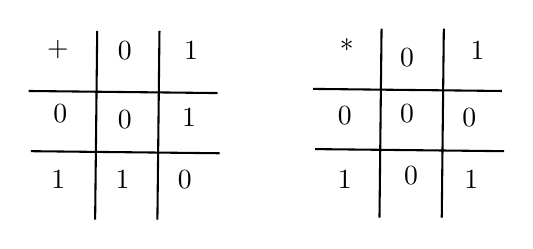
\begin{tikzpicture}[x=0.75pt,y=0.75pt,yscale=-1,xscale=1]
%uncomment if require: \path (0,350); %set diagram left start at 0, and has height of 350

%Shape: Boxed Line [id:dp6291595595512527] 
\draw    (288.6,132) -- (197.6,131) ;
%Straight Lines [id:da0037758895887590738] 
\draw    (230.6,102) -- (229.6,193) ;
%Straight Lines [id:da8491580753688753] 
\draw    (260.6,102) -- (259.6,193) ;
%Shape: Boxed Line [id:dp07775959649029429] 
\draw    (289.6,161) -- (198.6,160) ;
%Shape: Boxed Line [id:dp8480833689358503] 
\draw    (425.6,131) -- (334.6,130) ;
%Straight Lines [id:da6845007899647696] 
\draw    (367.6,101) -- (366.6,192) ;
%Straight Lines [id:da890039541275841] 
\draw    (397.6,101) -- (396.6,192) ;
%Shape: Boxed Line [id:dp9051592988280287] 
\draw    (426.6,160) -- (335.6,159) ;

% Text Node
\draw (346,104.1) node [anchor=north west][inner sep=0.75pt]    {$*$};
% Text Node
\draw (205,105.1) node [anchor=north west][inner sep=0.75pt]    {$+$};
% Text Node
\draw (239,105.9) node [anchor=north west][inner sep=0.75pt]   [align=left] {0};
% Text Node
\draw (208,135.9) node [anchor=north west][inner sep=0.75pt]   [align=left] {0};
% Text Node
\draw (345,136.9) node [anchor=north west][inner sep=0.75pt]   [align=left] {0};
% Text Node
\draw (375,108.9) node [anchor=north west][inner sep=0.75pt]   [align=left] {0};
% Text Node
\draw (207,167.9) node [anchor=north west][inner sep=0.75pt]   [align=left] {1};
% Text Node
\draw (271,105.9) node [anchor=north west][inner sep=0.75pt]   [align=left] {1};
% Text Node
\draw (345,167.9) node [anchor=north west][inner sep=0.75pt]   [align=left] {1};
% Text Node
\draw (409,105.9) node [anchor=north west][inner sep=0.75pt]   [align=left] {1};
% Text Node
\draw (270,137.9) node [anchor=north west][inner sep=0.75pt]   [align=left] {1};
% Text Node
\draw (238,167.9) node [anchor=north west][inner sep=0.75pt]   [align=left] {1};
% Text Node
\draw (406,167.9) node [anchor=north west][inner sep=0.75pt]   [align=left] {1};
% Text Node
\draw (239,138.9) node [anchor=north west][inner sep=0.75pt]   [align=left] {0};
% Text Node
\draw (268,167.9) node [anchor=north west][inner sep=0.75pt]   [align=left] {0};
% Text Node
\draw (375,135.9) node [anchor=north west][inner sep=0.75pt]   [align=left] {0};
% Text Node
\draw (405,137.9) node [anchor=north west][inner sep=0.75pt]   [align=left] {0};
% Text Node
\draw (377,165.9) node [anchor=north west][inner sep=0.75pt]   [align=left] {0};
\end{tikzpicture}
\newline
$\to (\mathbb{Z}_2,+,\cdot)$ es un campo. 
\item Sea $P=\s{0}$. \newline (1) Cumple (2) Cumple (3) No cumple $\to P$ no es una clase positiva de $\mathbb{Z}_2$.
\item Sea $P'=\s{1}$\newline (1) No cumple. $\to P'$ no es una clase positiva de $\mathbb{Z}_2$.
\end{itemize}
\end{example}

\begin{definition}
Sea $P$ la clase positiva del campo $\mathbb{F}$, entonces se dice que $\mathbb{F}$ está ordenada por $P$. (O que $\mathbb{F}$ es un campo ordenado).
\begin{itemize}
    \item Si $a\in P$, se dice que $a$ es positivo. Notación $a>0$. 
    \item Si $a\in P$ o $a=0$, se dice que $a$ es no negativo. Notación $a\geq 0$
    \item Si $a,b \in \mathbb{F}$ y $a-b\in P$, se escribe $a>b$.
    \item Si $a,b\in \mathbb{F}$ y $a-b\in P$ o $a-b=0$, se escribe $a\geq b$. 
\end{itemize}
\end{definition}

\begin{proposition}
Algunas propiedades...
\begin{itemize}
    \item{Transitividad} Si $a>b$ y $b>c\to a>c$.
    \item{Tricotomía} Si $a,b\in \mathbb{F}$, entonces: \newline $a>b\quad\quad O_{ex}\quad\quad a=b \quad \quad O_{ex}\quad \quad b>a$.
    \item{Antisimetría} Si $a\geq b$ y $b\geq a \to a=b$
\end{itemize}
\end{proposition}
\begin{proof}
Se presentan las pruebas: 
\begin{itemize}
    \item {1.} Si $$a>b\to a-b\in P$$
                  $$b>c\to b-c \in P$$
                  $$\to (a-b)+(b-c)= a-c \in P$$
                  $$\to a>c$$
    \item {2.} Por la tricotomía en $P$.
    \item {3.} Supóngase, por el absurdo, que $a\geq b$, $b\geq a$ y $a\neq b$. Entonces $a>b\quad \quad O_{ex} \quad \quad b>a (\to\gets)$
\end{itemize}
\end{proof}
\begin{proposition}
Sea $\mathbb{F}$ un campo ordenado: 
\begin{itemize}
    \item Si $a\neq 0\to a^2>0$
    \item 1>0
    \item Si $n\in \mathbb{Z}^+\to n>0$
\end{itemize}
\end{proposition}

\begin{proof}
Pruebas\\
\textbf{1.}
\begin{itemize}
\item Si $a\neq 0 \to a>0\quad\quad O_{ex}\quad \quad a<0$.
\item Si $a>0\to a\cdot a= a^2 >0$\\ (Por la propiedad de $a\in P \to a\cdot a \in P \to a^2>0$).
\item Si $a<0 \to -a\in P\to (-a)\cdot (-a) = a^2\in P\to a^2>0$.
\end{itemize}
\textbf{2.}
\begin{itemize}
    \item Hacemos $a=1$ en 1) $\to 1^2=1>0$. 
\end{itemize}
\textbf{3.} Por inducción sobre $n$.
\begin{itemize}
    \item Probemos para $n=1$. Por 2), $1>0$.
    \item Suponemos que $k>0$.
    \item Probamos para $k+1$; $k>0,1>0 \to k+1>0\to n>0, \forall n\in \mathbb{Z}^+$
\end{itemize}
\end{proof}

\begin{theorem}
Sean $a,b,c\in \mathbb{F}$...
\begin{itemize}
    \item  Si $a>b\to a+c>b+c$
    \item Si $a>b$ y $c>d\to a+c>b+d$
    \item Si $a>b$ y $c>0\to a\cdot c >b\cdot c$
    \item Si $a>b$ y $c<0\to a\cdot c<b\cdot c$
    \item Si $a>0\to a^{-1}>0$
    \item Si $a<0\to a^{-1}<0$
\end{itemize}
\end{theorem}
\begin{proof}
Prueba...
\begin{enumerate}
    \item Si $a>b\to a-b\in P\leftrightarrow (a+c)-(b+c)\in P\to a+c >b+c$.
    \item Si $$a>b\to a-b\in P$$
    $$c>d\to c-d \in P $$ $$\to (a-b)+(c-d)=(a+c)-(b+c)\in P$$
    $$\to a+c >b+c$$
    \item Si $$a>b\to a-b\in P$$
    $$c>0 \to c\in P$$
    $$\to (a-b)\cdot c = ac-bc\in P\to ac>bc $$
    \item Si $$a>b\to a-b\in P$$
            $$c<0 \to -c\in P$$
            $$\to (a-b)\cdot (-c)= bc-ac\in P$$
            $$\to bc>ac$$
    \item Sea $a>0$ y suponemos $a^{-1}<0\to -a^{-1}>0 \to a(-a^{-1})>0$, pero $a(-a^{-1})=-1>0(\to\gets)$. Si $a^{-1}=0\to 1=aa^{-1}=0 (\to\gets)\to a^{-1}>0$. 
    \item Similar al 5) 
\end{enumerate}
\end{proof}

\begin{corollary}
Si $a>b\to a>\frac{a+b}{2}>b$
\end{corollary}

\begin{proof}
\begin{align}
    \mi{a>b &\to a+a>a+b}\\
    \mi{&\to 2a>a+b}\\
    \mi{&\to a>\frac{a+b}{2}}
\intertext{Por otro lado}
    \mi{a>b &\to a+b>b+b}\\
    \mi{&\to a+b>2b}\\
    \mi{&\to \frac{a+b}{2}>b}\\
\mi{&\therefore a>\frac{a+b}{2}>b}
\end{align}
\marginnote[-12   pt ]{En el corolario, hagamos $b=0$. Entonces, si $a>0\implies a>\frac{a}{2}>0$. Entonces, en un campo ordenado no existe un número positivo menor.}
\end{proof}

\begin{theorem}
Si $ab>0$, entonces, $a>0$ y $b>0$ o $a<0$ y $b<0$.
\end{theorem} 

\begin{proof}
Pendiente
\end{proof}

\subsection{Valor absoluto}
\begin{definition}
Sea $\mathbb{F}$ un campo con clase positiva $P$. Se define la función valor absoluto: 
$$|\cdot|: \mathbb{F}\to P \cup \s{0}\ni $$
$$|a|=\begin{cases} 
      a & \text{si } a\geq 0 \\
      -a & \text{si } a<0
   \end{cases}$$
\end{definition}

\begin{theorem}
Related
\begin{enumerate}
    \item $|a|=0$ ssi $a=0$
    \item $|-a|=|a|$
    \item $|ab|=|a|\cdot|b|$
    \item Si $c\geq 0\to |a|\leq c$ ssi $-c\leq a\leq c$
\end{enumerate}
\end{theorem}

\begin{proof}
Pruebas...
\begin{enumerate}
    \item 
    ($\to$) Si $a=0\to$ Por definición: $|a|=|0|=0$.
    \newline 
    ($\gets$) A probar: Si $|a|=0\to a=0$
    \newline 
    \textit{Por contrapuesta,} suponga que $a\neq 0\to a>0$ o $a<0$.  
    \newline 
    Si $a>0\to |a|=a>0\to |a|\neq 0$
    \newline 
    Si $a<0\to |a|=-a>0= |a|\neq 0$
    \newline 
    i.e. si $a\neq 0\to |a|= 0$
    \item A probar: $-|a|=|a|$
    \newline
    Si $a>0\to |a|=a=|-a|$
    \newline 
    Si $a<0\to |a|=-a=|-a|$
    \newline 
    Si $a=0\to |0|=0=|-0|$
    
    \item $|ab|=|a|\cdot |b|$\newline 
    Por casos:
    \begin{itemize}
        \item Si $a>0$ y $b>0$, entonces: $$ab>0\to |ab|=ab=|a|\cdot |b|$$
        \item Si $a>0$ y $b<0\to ab<0\to |ab|=-(ab)=a\cdot (-b)=|a|\cdot |b|$
        \item Si $a<0$ y $b<0\to ab>0\to |ab|=ab=(-a)(-b)=|a|\cdot |b|$
    \end{itemize}
    \item A probar: si $c\geq 0\to |a|\leq c$ ssi $-c\leq a\leq c$
    \marginnote[-12   pt ]{$a\leq b\qquad -a\leq b \leftrightarrow |a|\leq b$}
    \newline 
    ($\to$) Suponga que $|a|\leq c\to a\leq c$ y $-a\leq c \to a\leq c$ y $a\geq -c, \therefore -c\leq a\leq c$
    \newline 
    ($\gets$) Suponga que $-c\leq a\leq c \to -c\leq a $ y $a\leq c\to c\geq -a$ y $a\leq c$ $\therefore |a|\leq c$
\end{enumerate}
\end{proof}


